\appendix
% \section{Combining noisy long-term context and clean short-term context}

% \label{sec:noise}
% \looseness=-1
% In this section, we explain our experiments and intuitions that led to the design of MAR.
% In preliminary experiments, music generation models trained with the MAR framework were diverging quickly during inference because they were not robust to error accumulations. 
% \citet{sony_trick} introduce a noise augmentation trick at training time in order to tackle this problem. Given a sequence $(\mathbf{x}^1, \mathbf{x}^2, \ldots, \mathbf{x}^S)$, they sample $k_s \sim \mathcal{U}(0, 1)$ and $\bm{\epsilon}_s \sim \mathcal{N}(0, \mathbf{I})$ for every $s \in \{1, \ldots, S\}$ and compute $\tilde{\mathbf{x}}^s = k_s  \bm{\epsilon}_s + (1 - k_s) \mathbf{x}^s$ for every $s$. After comparison and to preserve the variance of the $\mathbf{x}^s$ that are gaussians, we modify the noising formula as follows: $\tilde{\mathbf{x}}^s = \sqrt{k_s}  \bm{\epsilon}_s + \sqrt{1 - k_s} \mathbf{x}^s$.

% \looseness=-1
% In our case, applying this noising method to music generation slightly improves model stability but often reduces detail and instrument diversity, typically preserving only rhythmic elements, with audio fading into silence after 10–15 seconds. Since \citet{sony_trick} targets short, single-instrument clips, it's unsurprising the method performs best in that constrained setting. We hypothesize that the added noise inhibits the backbone transformer from encoding fine-grained information into $\mathbf{z}^s_{\text{long}}$, limiting the MLP’s ability to reconstruct detailed audio. However, combining this with a short-context transformer computing $\mathbf{z}^s_{\text{short}}$ yields the best results (Tab.~\ref{tab:ablation_fad}), likely because the clean short-term context restores local detail needed to model the distribution of the next $\mathbf{x}^s$.


\section{Lagrangian Self-Distillation}
\label{sec:LSD}
Lagrangian Self-Distillation (LSD) \citep{lsd} extends the consistency-model framework by introducing an additional time parameter $s$, enabling the model to learn mappings between arbitrary points along the probability flow trajectory rather than only from noisy inputs to clean data. An LSD model is a neural network $f_\phi(\mathbf{x}, t, s)$ that predicts the state of the PF-ODE solution at time $s$ given its state $\mathbf{x}_t$ at time $t$: $\forall (s,t) \in[0,1]^2, f_\phi(\mathbf{x}_t, t, s)=\mathbf{x_s}$.
In particular, with $t=1, s=0$ and by sampling $\mathbf{x}_1 \sim \mathcal{N}(0, I)$ we can sample from the data distribution with $f_\phi(\mathbf{x}_1, t=1, s=0)$.

In \citep{lsd}, the authors define $\mathbf{F}_\phi(\mathbf{x}, t, s)$ as 
\begin{equation}
    f_\phi(\mathbf{x}, t, s) = \mathbf{x} + (s - t) F_\phi(\mathbf{x}, t, s).
\end{equation}

To train a LSD model from scratch we need to combine a flow matching loss as well as a LSD loss: $\mathcal{L} = \mathcal{L}_{FM} + \mathcal{L}_{LSD}$. With an adaptive weighting loss $w_\psi(t, s)$ and our notations they derive as:
\begin{equation}
    \mathcal{L}_{\text{FM}}(\phi, \psi) = \mathbb{E}_{\mathbf{x}_0 \sim p_{\text{data}},\, \bm{\epsilon} \sim \mathcal{N}(0, \mathbf{I}),\, t \sim \mathcal{U}(0, 1)}
\left[ e^{-w_\psi(t, t)} \left\| F_\phi(\mathbf{x}_t, t, t) - \left( \alpha'_t \mathbf{x}_0 + \sigma'_t \bm{\epsilon} \right) \right\|_2^2 + w_\psi(t, t)\right].
\end{equation}
and
\begin{equation}
    \mathcal{L}_{\text{LSD}}(\phi, \psi) = \mathbb{E}_{\mathbf{x}_0, \bm{\epsilon}, t,s}
\left[ e^{-w_\psi(t, s)} \left\| \partial_sf_\phi(\mathbf{x}_t, t, s) - F_{\phi^-}(f_\phi(\mathbf{x}_t, t, s), s, s) \right\|_2^2 + w_\psi(t, s)\right].
\end{equation}

 where $\mathbf{x}_0 \sim p_{\text{data}},\, \bm{\epsilon} \sim \mathcal{N}(0, \mathbf{I}), t \sim \mathcal{U}(0, 1), s \sim \mathcal{U}(0, t)$.

 In practice, we compute the flow matching loss on 75\% of a batch and the LSD loss on the 25\% left. 


\section{Our Music VAE}
\label{sec:music_vae}
\begin{table}[h]
\caption{\textbf{Music compression models.} At least 96 VAE latent dimensions are required to outperform the 32-RVQ codec on reconstruction metrics. EnCodec has been retrained on our dataset.}
\centering
\scriptsize % smaller font
\setlength{\tabcolsep}{4pt} % tighter column spacing
\renewcommand{\arraystretch}{0.95} % tighter row spacing
\begin{tiny}
\begin{sc}

\begin{tabular}{lrrrrr}
\toprule
\textbf{Model Type} & \textbf{Dims / RVQ} & \textbf{Frame Rate (Hz)} & \textbf{Bitrate (kbps)} & \textbf{VisQOL} ($\uparrow$) & \textbf{SISNR} ($\uparrow$) \\
\midrule
EnCodec \cite{musicgen}
 & 4 RVQ & 50 & 2.2 & 2.41 & 5.62 \\
VQ-VAE (inspired from Mimi) & 32 RVQ & 25 & 8.8 & 3.63 & 9.61 \\
VAE & 32 dims  & 25 & --  & 2.23 & 5.51 \\
VAE & 96 dims  & 25 & --  & 3.65 & 9.76 \\
VAE & 128 dims & 25 & --  & \textbf{4.01} & \textbf{10.3} \\
\bottomrule
\end{tabular}
%}
\end{sc}
\end{tiny}
\label{tab:visqol}
\end{table}

\looseness=-1
Our variational autoencoder (VAE) and codec architecture is adapted from the Mimi codec \citep{moshi}, originally designed for 24kHz speech at 12.5Hz. We trained it to compress 32kHz mono music with a 25Hz frame rate. We experiment with bottleneck sizes of 96 and 128 dimensions. For comparison, MusicGen's EnCodec model \citep{musicgen} also operates at 32kHz but uses a 4-level RVQ at 50Hz. In Tab.~\ref{tab:visqol}, we report reconstruction metrics (audio ViSQOL \cite{visqol} and SISNR), showing that a 32-dim VAE matches MusicGen's codec, and that at least 96 dimensions are needed for our VAE to match the quality of the 32-level RVQ configuration.

\section{Effect of gaussian temperature sampling}
\label{sec:effect_temp}
\looseness=-1
We evaluate how our proposed gaussian temperature sampling method affects acoustic diversity for consistency models, in comparison with temperature sampling on its discrete counterpart.  More precisely, we compute WavLM speaker embeddings~\citep{wavlm} over 100 unprompted speech generations with different values of temperature, both for an RQ-transformer and CALM. In both cases, the inner monologue text stream is generated with 0.8 temperature to ensure text diversity. We then average the pairwise cosine similarities of these embeddings, as a measure of diversity: the higher the average similarity, the lower speaker diversity in generated audio. The reference speaker similarity number is computed over 100 examples from the ground truth dataset. Fig.~\ref{fig:speaker_sim} shows, as expected, that speaker similarity tends to decrease with temperature, which means that temperature increases diversity with a similar trajectory to the discrete models. 

\begin{figure}[H]
  \centering
  \begin{minipage}[c]{0.74\linewidth}
    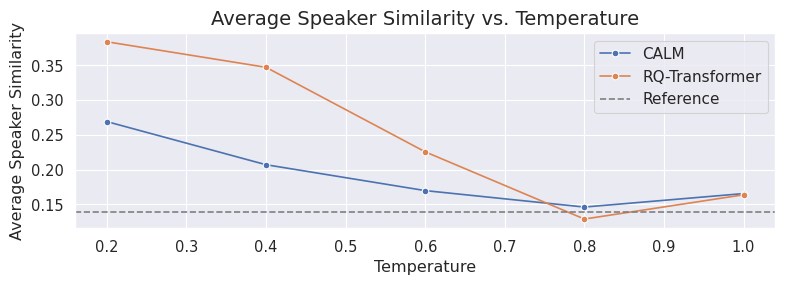
\includegraphics[width=\linewidth]{speaker_sim_calm.png}
  \end{minipage}%
  \hfill
  \begin{minipage}[c]{0.24\linewidth}
    \caption{\small Average pairwise speaker similarity over 100 unprompted 10s generations, or 100 10s examples from the ground truth dataset as reference. As expected, for both methods models generate more diverse speakers (i.e. less pairwise speaker similarity) as temperature increases.}
    \label{fig:speaker_sim}
  \end{minipage}
\end{figure}


\section{Data used for the text-to-speech model}
\label{sec:tts_data}
The dataset used to train our TTS models is composed of AMI \cite{carletta2007ami}, 
EARNINGS22 \cite{delrio2022earnings22}, 
GIGASpeech \cite{chen2021gigaspeech}, 
SPGISpeech \cite{oneill2021spgispeech}, 
TED-LIUM \cite{hernandez2018tedlium3}, 
VoxPopuli \cite{wang2021voxpopuli}, 
LibriHeavy \cite{libriheavy2024}, 
and Emilia \cite{emilia2023}. It results into 88k hours of audio. 


\section{Supplementary Experiments}
\subsection{Head batch multiplier value}

\begin{figure}[H]
\centering
\begin{minipage}{0.5\textwidth}
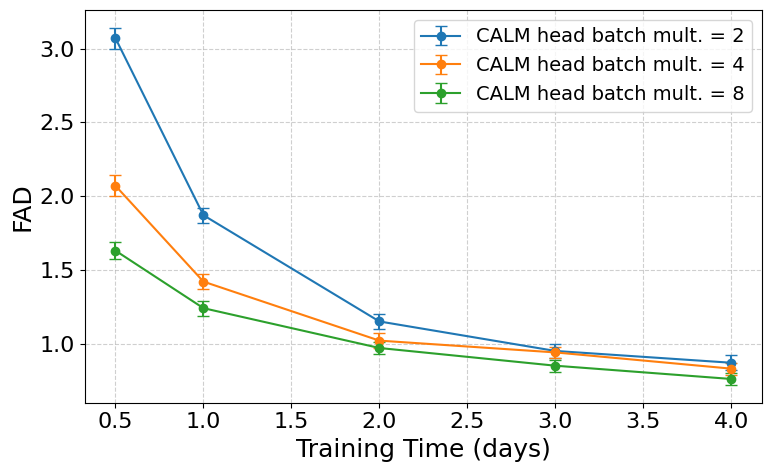
\includegraphics[width=\linewidth]{head_batch.png}
\end{minipage}%
\begin{minipage}{0.5\textwidth}
\caption{\textbf{Effect of the head batch multiplier value.} Training a model (music consistency CALM) with a higher batch size multiplier fastens the convergence for the FAD metric. All the evaluations are done with 4 steps of consistency at inference time.}
\label{fig:head_batch_multiplier}
\end{minipage}
\end{figure}



\subsection{Short-context transformer window}
\label{sec:K_hyperparameter}
To study the influence of the context window $K$ of the short-context transformer, we performed an hyperparameter search with $K=5, 10, 20, 40$ and trained our models for 500K training steps (see Tab.~\ref{tab:K_short_context_transformer}). The model is the music continuation CALM and all evaluations are done with 4-steps of consistency. We observe that finding an optimal value of $K$ is not critical even though it seems that 5 is too small enough. 

\begin{table}[h]
\centering
\caption{\textbf{FAD after 500K training steps for different short-context Transformer contexts} $K$.}
\begin{tabular}{lc}
\toprule
$K$ in short-context Transformer & FAD \\
\midrule
5  & $0.85 \pm 0.05$ \\
10 & $0.76 \pm 0.04$ \\
20 & $0.73 \pm 0.04$ \\
40 & $0.78 \pm 0.04$ \\
\bottomrule
\end{tabular}
\label{tab:K_short_context_transformer}
\end{table}

\subsection{Comparison of TrigFlow and Consistency on inference speed and quality criteria}
\label{sec:num_steps}
In Tab.~\ref{tab:num_steps} we compare the inference speed for both TrigFlow CALM and Consistency CALM on the task of music continuation on our test set. We see that below the 10 steps regime, only the Consistency model performs well. Moreover, around 10 steps is the limit for streaming applications where the real time factor (RTF) is smaller than 1. This justifies the need of consistency modeling (instead of diffusion or flow matching) for good quality streaming generation.

\begin{table}[h]
\caption{ \textbf{Generation efficiency of TrigFlow CALM and Consistency CALM models.} 
We compute the inference time to generate 30 seconds of audio, the corresponding Real Time Factor (RTF) as well as the FAD metric for different numbers of inference steps. For streaming (RTF<1), only consistency generates good quality audio.}
\centering
\renewcommand{\arraystretch}{1.1}

\begin{tabular}{lcccc}
\toprule
\textbf{\# Steps} & \textbf{Time (s)} & \textbf{RTF} & \textbf{FAD (TrigFlow)} & \textbf{FAD (Consistency)} \\
\midrule
1   & 16.7  & $0.56$ & --            & $0.83 \pm 0.04$ \\
4   & 20.4  & $0.68$ & $28.83 \pm 0.20$ & $0.71 \pm 0.05$ \\
10  & 27.7  & $0.92$ & $4.62 \pm 0.07$  & $0.73 \pm 0.05$ \\
25  & 46.1  & $1.54$ & $0.79 \pm 0.04$  & $0.96 \pm 0.06$ \\
50  & 76.8  & $2.56$ & $0.74 \pm 0.05$  & $1.46 \pm 0.06$ \\
100 & 136.4 & $4.55$ & $0.64 \pm 0.04$  & $2.05 \pm 0.07$ \\
\bottomrule
\end{tabular}

\label{tab:num_steps}
\end{table}

\subsection{Scalability of CALM}
\label{sec:scalability}
In order to see if all the hyperparameters of our CALM method transfer well to more model parameters, we trained a consistency music CALM model with a larger 3B backbone (with a model dimension of 2048, 32 heads and 48 layers) as well as a discrete RQ-Transformer with 32-RVQ model with the same backbone size. For the CALM model, we use 4 consistency steps at inference. Tab.~\ref{tab:scalability} shows that the FAD are improving with a bigger backbone (3B vs 1.3B) in similar proportions for both discrete-based (RQ-Transformer) and continuous-based (CALM) models. 


\begin{table}[h]
\centering
\caption{\textbf{Scalability of the backbone for CALM and RQ-Transformer methods.}}
\begin{tabular}{lc}
\toprule
\textbf{Model} & \textbf{FAD} \\
\midrule
CALM with 3B backbone & $0.62 \pm 0.05$ \\
32 RVQ RQ-Transformer with 3B backbone & $0.98 \pm 0.06$ \\
CALM with 1.3B backbone & $0.71 \pm 0.05$ \\
32 RVQ RQ-Transformer with 1.3B backbone & $1.06 \pm 0.06$ \\
\bottomrule
\end{tabular}
\label{tab:scalability}
\end{table}


\subsection{Text-to-Speech ablation study}

\resizebox{\textwidth}{!}{% <--- Starts the resize to fit \textwidth
\begin{tiny}
\begin{sc}
\begin{tabular}{lcrrrrrrr}
\toprule
\textbf{Model} & \textbf{Num. parameters} & \textbf{WER} & \textbf{CER}& \textbf{SIM} & \textbf{MUSHRA} & \textbf{Speaker SIM} \\
& & ($\downarrow$) & ($\downarrow$) & ($\uparrow$) & ($\uparrow$) & \textbf{(Human eval ELO} ($\uparrow$) \\
\midrule
CALM w/ LSD (NFE=1, CFG=1.5 w.r.t text) & 313M & 1.81 & 0.57 & 0.52 & 61.1 $\pm$ 2.3 & 1966 $\pm$ 23 \\
CALM w/ LSD (NFE=1, no CFG) & 313M & 2.39 & 0.90 & 0.52 & 55.5 $\pm$ 2.2 & 1991 $\pm$ 26 \\
CALM w/ LSD (NFE=1, CFG=1.25 w.r.t text and audio prefix) & 313M & 1.86 & 0.59 & 0.54 & 56.2 $\pm$ 2.2 & 1995 $\pm$ 27 \\
CALM w/ Consistency (NFE=1, CFG=1.5 w.r.t text) & 313M & 1.93 & 0.62 & 0.40 & 46.8 $\pm$ 2.5 & 1900 $\pm$ 30 \\
\bottomrule
\end{tabular}
\end{sc}
\end{tiny}
}

We can see in Tab.~\ref{tab:scalability} that at this smaller scale ($\sim$300M), Lagrangian Self-Distillation models provide better audio quality than Consistency models. We also conclude that the latent CFG has a significant impact over the WER. As well, applying the latent CFG on the audio prefix improves the speaker similarity but at the cost of audio quality.
All models were run with sampling from a Gaussian with 0.7 temperature (i.e., multiplying the standard Gaussian noise by $\sqrt{0.7}$).

\subsection{Text-to-Music evaluation on MusicCaps}
\label{sec:text-to-music}
We report the results on the MusicCaps dataset \cite{musiclm} and report as well the results of MusicLM \citep{musiclm}, the original text-to-music MusicGen Medium \citep{musicgen}, AudioLDM2 \citep{audioldm2}, Noise2Music \citep{noise2music}, Jen-1 \citep{jen1} as well as MusicFlow \citep{musicflow} on the FAD, the KL Divergence (KLD) metric based on the pre-trained audio model PANN \citep{pann} as well as the CLAP cosine similarity that measures the matching between the generated music and text description. The results of Tab.~\ref{tab:text_to_music} show that even though our goal is not to specifically build the best text-to-music model, simply applying CALM on our dataset with a CLAP conditioning leads to competitive results. The metrics from the models that we did not train are reported from the MusicFlow \citep{musicflow} paper.


% \begin{table}[h]
% \caption{{Text-to-music results on the MusicCaps dataset.}}
% \centering
% \resizebox{\textwidth}{!}{%
% \begin{sc}
% {
% \begin{tabular}{lcccc}
% \toprule
% \textbf{Model} & \textbf{\# params} & \textbf{FAD} ($\downarrow$) & \textbf{KLD} ($\downarrow$) & \textbf{CLAP} ($\uparrow$) \\ %& --  \\
% \midrule
% Reference & -- & -- & -- & 0.30 \\ %& --  \\
% \midrule
% MusicLM \citep{musiclm}& 860M & 4.00 & -- & -- \\ %& --  \\
% MusicGen Medium \citep{musicgen}& 1.5B & 3.40 & 1.23 & 0.37 \\ %& --  \\
% AudioLDM2 \citep{audioldm2}& 746M & 3.13 & 1.20 & 0.43 \\ %& --  \\
% Noise2Music \citep{noise2music}& 1.3B & 2.10 & -- & -- \\ %& --  \\
% Jen-1 \citep{jen1}& 746M & 2.00 & 1.29 & -- \\ %& --  \\
% MusicFlow (Unidirectional LM + FM) \citep{musicflow}& 546M & 2.69 & 1.23 & 0.52 \\ %& --  \\
% \midrule
% MusicGen Medium (retrained with CLAP)& 1.5B & 2.70 & 1.37 & 0.39 \\ %& --  \\
% RQ-transformer 32 RVQ & 2.05B & 2.56 & 1.35 & 0.43 \\ %& --  \\
% CALM - Consistency - 4 Steps& 1.95B & 2.14 & 1.30 & 0.44 \\ %& --  \\
% \bottomrule
% \end{tabular}
% }
% \end{sc}
% }
% \label{tab:text_to_music}
% \end{table}

\begin{table}[h]
\caption{{Text-to-music results on the MusicCaps dataset.}}
\centering
\resizebox{\textwidth}{!}{%
\begin{sc}
{
\begin{tabular}{lccc}
\toprule
\textbf{Model} & \textbf{FAD} ($\downarrow$) & \textbf{KLD} ($\downarrow$) & \textbf{CLAP} ($\uparrow$) \\
\midrule
Reference & -- & -- & 0.30 \\
\midrule
MusicLM \citep{musiclm} & 4.00 & -- & -- \\
MusicGen Medium \citep{musicgen} & 3.40 & 1.23 & 0.37 \\
AudioLDM2 \citep{audioldm2} & 3.13 & 1.20 & 0.43 \\
Noise2Music \citep{noise2music} & 2.10 & -- & -- \\
Jen-1 \citep{jen1} & 2.00 & 1.29 & -- \\
MusicFlow (Unidirectional LM + FM) \citep{musicflow} & 2.69 & 1.23 & 0.52 \\
\midrule
MusicGen Medium (retrained with CLAP) & 2.70 & 1.37 & 0.39 \\
RQ-transformer 32 RVQ & 2.56 & 1.35 & 0.43 \\
CALM - Consistency - 4 Steps & 2.14 & 1.30 & 0.44 \\
\bottomrule
\end{tabular}
}
\end{sc}
}
\label{tab:text_to_music}
\end{table}

\section{Pocket TTS}
\label{sec:pocket_tts}
Given a 313M parameters text-to-speech CALM model that has a 24 layers backbone transformer (the teacher), we do latent distillation to a 6 layers transformer backbone (the student) and a CFG coefficient of $\alpha=1.5$ applied to the teacher. We keep the same MLP sampling head. The final model, named \textbf{Pocket TTS} has a size of 90M parameters while the VAE has 20M parameters. In Tab.\ref{tab:pocket-tts}, we put 100M parameters to include the VAE decoder in the parameter count. 

We evaluate Pocket TTS on the Librispeech test-clean set following the same protocol as F5-TTS \citep{f5tts}, with the difference that we cleaned the audio input using Adobe Enhance Speech\footnote{\url{https://podcast.adobe.com/en/enhance}} to obtain 24kHz high-quality audio. We evaluate all baselines with the enhanced samples\footnote{\url{https://huggingface.co/datasets/kyutai/librispeech_test_clean_enhanced }}. 

We compare against three baselines: F5-TTS \citep{f5tts}, DSM \citep{delayed_stream_modeling}, Chatterbox Turbo\footnote{\url{https://www.resemble.ai/chatterbox-turbo/}} and Kokoro TTS\footnote{\url{https://huggingface.co/hexgrad/Kokoro-82M}}. We report Word Error Rate (WER) using Whisper-large-v3\citep{whisper}, as well as the results of a pairwise human evaluation for audio quality and speaker similarity. For audio quality, we ask raters “Which of the two audio clips has the best audio quality?”, and for speaker similarity, we ask “Which of the two audio clips sounds more similar to the reference audio clip in terms of voice characteristics?” and provide the voice prompt as a reference.

\begin{table}[h]
\caption{{Comparison of TTS models on Librispeech test-clean.}}
\centering
\resizebox{\textwidth}{!}{%
\begin{sc}
{
\begin{tabular}{lcccccc}
\toprule
\textbf{Model} &
\textbf{Param size} &
\textbf{WER} &
\textbf{Audio Quality} &
\textbf{Speaker Sim} &
\textbf{Faster than} \\
&
\textbf{(gen. only)} &
($\downarrow$) &
\textbf{(ELO)} ($\uparrow$) &
\textbf{(ELO)} ($\uparrow$) &
\textbf{real-time CPU} \\
\midrule
F5-TTS \citep{f5tts} & 336M & 2.21 & $1949 \pm 27$ & $1946 \pm 26$ & $\times$ \\
DSM & 750M & 1.84 & $1959 \pm 25$ & $2037 \pm 21$ & $\times$ \\
Chatterbox Turbo & 350M & 3.24 & $2055 \pm 23$ & $2012 \pm 22$ & $\times$ \\
\midrule
Kokoro & 82M & 1.93 & \multicolumn{2}{c}{No voice cloning} & $\checkmark$ \\
\midrule
\textbf{Pocket TTS (ours)} & \textbf{100M} & \textbf{1.84} & \textbf{$2016 \pm 25$} & \textbf{$1898 \pm 26$} & $\checkmark$ \\
\bottomrule
\end{tabular}
}
\end{sc}
}
\label{tab:pocket-tts}
\end{table}

As seen in Tab.~\ref{tab:pocket-tts}, Pocket TTS has the lowest Word Error Rate, a better Audio Quality than the ground truth F5-TTS and DSM, as well as an on-par Speaker Similarity with the ground truth while being a significantly smaller model than competitors, and being the only one that can run faster than real-time on CPU (we tested on Apple M3 and Intel core ultra 7 165H). We invite the reader to check the blog post where the one-line installation of the model is provided: \href{https://kyutai.org/pocket-tts-technical-report}{kyutai.org/pocket-tts-technical-report}.


\section{Human evaluation methods}
\label{sec:human_evals}
Audio clips are always 30s second total, with a 3s prompt coming from a ground truth audio. Each experiments has 50 samples for each method. There are 50 raters. Each of them sees 10 samples.
Raters were payed £9 / hour for their contribution.

\subsection{Speech continuation}
\textbf{Acoustic quality assessment}: How would you rate the overall quality of this audio clip? Consider aspects such as clarity, balance, richness, and naturalness. Listen to at least 10 seconds of audio before deciding.
1 clip is presented, possibilities are bad, poor, fair, good, excellent.

\textbf{Meaningfulness}: Which of these two audio clips feels more like meaningful and natural speech? The first 3 seconds are identical. Listen to at least 10 seconds of each clip.
2 clips are presented, ties are possible.
Elo scores are Bayesian estimates of the posterior mean in a Bradley-Terry model.


\subsection{Music continuation and CLAP-to-music}
\textbf{Acoustic quality assessment}: How would you rate the overall quality of this music? Consider aspects such as clarity, balance, richness, and naturalness. Listen to at least 10 seconds of audio before deciding.
1 clip is presented, possibilities are bad, poor, fair, good, excellent.

\textbf{Music enjoyment}: Which music do you enjoy listening to more? The first 3 seconds are identical. Listen to at least 10 seconds of each clip.
2 clips are presented, ties are possible.
Elo scores are Bayesian estimates of the posterior mean in a Bradley-Terry model.


% \textbf{Coherence}: How do you rate the coherence between the reference and each example? Each example is a continuation of the 3 second reference. How well do the examples match the reference?
% 5 clips are presented in addition to the reference prompt, and are rated between 0 and 100.

\subsection{Bayesian Elo Score}
The Meaningfulness metric for speech and the Enjoyment metric for music are both Bayesian Elo Scores. Elo score is used to rank models based on some pairwise comparisons of audio samples. Given two models $A$ and $B$, the probability that $A$ is preferred over $B$ is:
\begin{equation}
    P(A>B) = \frac{1}{1 +10^{(E_B-E_A)/400}}
    \label{eq:elo}
\end{equation}
where $E_A$ and $E_B$ are the Elo scores of each model. Unlike a traditional Elo score, the Bayesian Elo score uses a Gamma prior,
so that one can derive confidence intervals over the posterior distribution.


By defining $S_A$ such as $E_A=400\log_{10}(S_A) + c$ with $c$ being a constant, we obtain:
\begin{equation}
    P(A>B) = \frac{S_A}{S_A+S_B}
\end{equation}
which is a Bradley-Terry \citep{bradley_terry} model. There are a few different methods to estimate the parameters of a Bradley-Terry model. We use the iterative one from \citep{carondoucet} where $S_A^0$ follows a Gamma prior with parameters $\alpha^0, \beta^0$. By denoting $w_A$ the number of times where method $A$ won against any other methods and $n_{AB}$ the number of times where $A$ and $B$ are compared, $S_A^t$ is computed with the following update rule until convergence:
\begin{equation}
    S_A^{t+1} = \frac{\alpha +w_A}{\beta +\sum_{B \neq A}\frac{n_{AB}}{S_A^t+S_B^t}}
\end{equation}

which is the mean of the Gamma distribution with updated parameters $\alpha_A^{t+1},\beta_A^{t+1}$:
\begin{equation}
    \alpha_A^{t+1} = \alpha^0 + w_A,\qquad
    \text{and}\qquad \beta_A^{t+1} = 
    \beta^0 + \sum_{B\neq A} \frac{w_{A,B}}{S_A^t + S_B^t}.
\end{equation}
Iterating over $t$ allows to reach a fix point, we run 30 of them,
once we have collected all the pairs.
We use $\alpha=0.1, \beta=0.1, c=2000$ so that in absence of any data, $S_A=1$ and $E_A = 2000$. Confidence interval are 95\% confidence interval according to the posterior (the 2.5th and 97.5th percentiles).

\section{Hyperparameters}
\label{sec:appendix_hyperarameters}
We present in Tab.~\ref{tab:vae_params} the parameters of the music and speech VAE used for CALMs. For CALMs and the RQ-Transformer based discrete LMs, the hyperparameters are presented in Tab.~\ref{tab:lm_params}.


% \begin{table}[H]
% %\begin{wraptable}{r}{6cm}
%   \centering
%   \caption{\label{tab:vae_params} VAE hyperparameters}
%   \footnotesize
%   %\resizebox{0.9\textwidth}{!}{
%   \begin{tabular}{l|c|c|c}
%     \toprule
%       &
%     \multicolumn{1}{c|}{Music VAE} &
%     \multicolumn{1}{c}{Speech continuation VAE} & \multicolumn{1}{c}{TTS VAE} \\
%     \midrule
%     \multicolumn{3}{c}{\textit{General}} \\
%     \midrule[0.3pt]
%     Sample rate    & 32kHz & 24kHz & 24kHz \\
%     Frame rate & 25Hz & 12.5Hz & 12.5Hz \\
%     Latent dimension & 128 & 32 & 32 \\
%     \midrule
%     \multicolumn{3}{c}{\textit{Architecture}} \\
%     \midrule[0.3pt]
%     Convolutions ratios   & 8, 8, 5, 4 & 6, 5, 4, 4, 4 & 120 before transformers and 16 after \\
%     Num transformer encoder layers & 4 & 8 & 8 \\
%     Num transformer decoder layers & 4 & 8 & 8 \\
%     Transformer context & 30s & 10s & 5s \\
%     \midrule
%     \multicolumn{3}{c}{\textit{Training parameters}} \\
%     \midrule[0.3pt]
%     Batch size & 64 & 64 & 64 \\
%     Audio sample length & 12s & 12s & 12s \\
%     KL loss weight & 0.01 & 0.01 & 0.01 \\
%     Reconstruction loss & \checkmark & \xmark & \checkmark then finetuned without \\
%     Distillation loss weight & \xmark & 25 & 25 \\
%     LR Schedule          & cosine & cosine & cosine \\
%     Learning rate      & $8 \cdot 10^{-4}$ & $8 \cdot 10^{-4}$ & $8 \cdot 10^{-4}$ \\
%     \bottomrule
%   \end{tabular}
% \end{table}


\begin{table}[H]
%\begin{wraptable}{r}{6cm}
  \centering
  \caption{\label{tab:vae_params} VAE hyperparameters}
  \footnotesize
  %\resizebox{0.9\textwidth}{!}{
  \begin{tabular}{l|c|c}
    \toprule
      &
    \multicolumn{1}{c|}{Music VAE} &
    \multicolumn{1}{c}{Speech continuation VAE}  \\
    \midrule
    \multicolumn{3}{c}{\textit{General}} \\
    \midrule[0.3pt]
    Sample rate    & 32kHz & 24kHz \\
    Frame rate & 25Hz & 12.5Hz \\
    Latent dimension & 128 & 32 \\
    \midrule
    \multicolumn{3}{c}{\textit{Architecture}} \\
    \midrule[0.3pt]
    Convolutions ratios   & 8, 8, 5, 4 & 6, 5, 4, 4, 4 \\
    Num transformer encoder layers & 4 & 8 \\
    Num transformer decoder layers & 4 & 8 \\
    Transformer context & 30s & 10s  \\
    \midrule
    \multicolumn{3}{c}{\textit{Training parameters}} \\
    \midrule[0.3pt]
    Batch size & 64 & 64  \\
    Audio sample length & 12s & 12s  \\
    KL loss weight & 0.01 & 0.01 \\
    Reconstruction loss & \checkmark & \xmark  \\
    Distillation loss weight & \xmark & 25  \\
    LR Schedule          & cosine & cosine \\
    Learning rate      & $8 \cdot 10^{-4}$ & $8 \cdot 10^{-4}$  \\
    \bottomrule
  \end{tabular}
\end{table}
\begin{table}[H]
\centering
\caption{\label{tab:lm_params} Model and training hyperparameters}
\footnotesize
\resizebox{\textwidth}{!}{%
\begin{tabular}{l|c|c|c}
  \toprule
  &
  \multicolumn{1}{c|}{Music} &
  \multicolumn{1}{c|}{Speech continuation} &
  \multicolumn{1}{c}{\textcolor{blue}{Text-to-Speech}} \\
  \midrule
  \multicolumn{4}{c}{\textit{Backbone Transformer}} \\
  \midrule[0.3pt]
  Model dimension    & 1536 & 2560 & \textcolor{blue}{1024} \\
  MLP dimension      & 6336 & 10560 & \textcolor{blue}{4096} \\
  Number of heads    & 24 & 20 & \textcolor{blue}{16} \\
  Number of layers   & 48 & 24 & \textcolor{blue}{24} \\
  Learning rate      & $1 \cdot 10^{-4}$ & $5 \cdot 10^{-5}$ & \textcolor{blue}{1e-4}\\
  Number of parameters & 1.35B & 2.2B & \textcolor{blue}{302M} \\
  \midrule
  \multicolumn{4}{c}{\textit{RQ-Transformer head (RVQ model)}} \\
  \midrule[0.3pt]
  Model dimension    & 1024 & 1024 & \textcolor{blue}{\xmark} \\
  MLP dimension      & 4096 & 4096 & \textcolor{blue}{\xmark} \\
  Number of heads    & 16 & 16 & \textcolor{blue}{\xmark} \\
  Number of layers   & 6 & 6 & \textcolor{blue}{\xmark} \\
  Number of parameters & 701M & 701M & \textcolor{blue}{\xmark} \\
  \midrule
  \multicolumn{4}{c}{\textit{Consistency sampler head (ours)}} \\
  \midrule[0.3pt]
  Number of layers & 12 & 6 & \textcolor{blue}{6} \\
  MLP dimension & 3072 & 512 & \textcolor{blue}{512} \\
  Gating & SiLU & SiLU & \textcolor{blue}{SiLU} \\
  Number of parameters & 601M & 10M & \textcolor{blue}{10M} \\
  \midrule
  \multicolumn{4}{c}{\textit{Short context transformer (ours)}} \\
  \midrule[0.3pt]
  Model dimension    & 1536 & \xmark & \textcolor{blue}{\xmark} \\
  MLP dimension      & 6336 & \xmark & \textcolor{blue}{\xmark} \\
  Number of heads    & 24 & \xmark & \textcolor{blue}{\xmark} \\
  Number of layers   & 4 & \xmark & \textcolor{blue}{\xmark} \\
  Context            & 10 & \xmark & \textcolor{blue}{\xmark} \\
  Number of parameters & 113M & \xmark & \textcolor{blue}{\xmark} \\
  \midrule
  \multicolumn{4}{c}{\textit{Audio embedding manipulations}} \\
  \midrule[0.3pt]
  Center and normalize    & \checkmark & \checkmark & \textcolor{blue}{\checkmark} \\
  Noise before entering backbone & \checkmark & \xmark & \textcolor{blue}{\xmark} \\
  \midrule
  \multicolumn{4}{c}{\textit{Training parameters}} \\
  \midrule[0.3pt]
  Head batch multiplier & 8 & 8 & \textcolor{blue}{8} \\
  Optimizer & AdamW $\beta_1=0.9, \beta_2=0.95$ & AdamW $\beta_1=0.9, \beta_2=0.95$ & \textcolor{blue}{AdamW $\beta_1=0.9, \beta_2=0.95$} \\
  Batch size & 48 & 144 & \textcolor{blue}{128} \\
  Audio sample length & 30s & 300s & \textcolor{blue}{60s} \\
  LR Schedule          & cosine & cosine & \textcolor{blue}{cosine} \\
  Learning rate      & $1 \cdot 10^{-4}$ & $2 \cdot 10^{-4}$ & \textcolor{blue}{1e-4} \\
  GPU used & 16 H100 & 48 H100 & \textcolor{blue}{8 H100} \\
  Number of training steps & 500k & 150k & \textcolor{blue}{400k} \\
  Initial checkpoint & \xmark & Helium-1 \citep{kyutai2025helium} & \textcolor{blue}{\xmark} \\
  Inner monologue      & \xmark & \checkmark & \textcolor{blue}{\xmark} \\
  Acoustic delay       & - & 2 frames (160 ms) & \textcolor{blue}{-} \\
  \bottomrule
\end{tabular}
} % end resizebox
\end{table}




